\chapter{Mecanismos de reacción: etapas elementales y aproximaciones}\label{ch:b1:elementary-steps}

El monóxido de nitrógeno, que se forma en los motores de los coches y en
los rayos, se combina con el oxígeno del aire: \ce{2NO + O2 -> 2NO2}.
Medida en el laboratorio, la velocidad de esta reacción es proporcional a
$[\ce{NO}]^2[\ce{O2}]$ --- y es \emph{más lenta} cuando se calienta el
gas. Un único choque de tres moléculas podría explicar el primer hecho,
nunca el segundo: todo choque gana energía con la temperatura. La
explicación es que la reacción no es un solo suceso, sino una secuencia
de sucesos más sencillos, su mecanismo. Este capítulo define esas \omterm{def:b1:elementary-steps:elementary-step}{etapas
elementales}, el \omterm{def:b1:elementary-steps:energy-profile}{perfil de energía} a lo largo del cual transcurren y las
aproximaciones que convierten un mecanismo en una \omterm{def:b1:rate-laws:order}{ley de velocidad};
termina con la catálisis, el arte de abrir un camino más fácil.

\begin{recall}
El libro 1 (año 12) describió un \omterm{def:b1:elementary-steps:elementary-step}{mecanismo de reacción} como una secuencia
de etapas dibujadas con flechas curvas, con intermedios que se forman y
se consumen, y un \omterm{def:b1:elementary-steps:catalyst}{catalizador} como una especie que acelera una reacción
sin consumirse. Las \omterm{def:b1:rate-laws:order}{leyes de velocidad}, los órdenes y la \omterm{thm:b1:rate-laws:arrhenius}{ley de Arrhenius}
se definieron en el
\cref{ch:b1:rate-laws}.
\end{recall}

\section{Etapas elementales}

\begin{definition}[Etapa elemental, molecularidad, mecanismo]\label{def:b1:elementary-steps:elementary-step}
Una \emph{etapa elemental}\index{etapa elemental} es una reacción que
tiene lugar en un único suceso molecular, tal como está escrita, sin
ningún intermedio. Su \emph{molecularidad}\index{molecularidad} es el
número de partículas que reaccionan en ese suceso: 1 (unimolecular, una
descomposición o una transposición), 2 (bimolecular, un choque), y rara
vez 3. Un \emph{mecanismo de reacción}\index{mecanismo de reaccion@mecanismo de reacción} es el
conjunto de etapas elementales cuya suma es la reacción global. Una
especie que se forma en una etapa y se consume en otra posterior, ausente
de la ecuación global, es un \emph{intermedio de
reacción}\index{intermedio de reaccion@intermedio de reacción}.
\end{definition}

\begin{proposition}[Ley de velocidad de una etapa elemental]\label{prop:b1:elementary-steps:elementary-law}
Una \omterm{def:b1:elementary-steps:elementary-step}{etapa elemental} admite un orden, y sus \omterm{def:b1:rate-laws:order}{órdenes parciales} son iguales
a sus coeficientes estequiométricos: $\mathrm{A} \to \dots$ tiene
$v = k[\mathrm{A}]$;
$\mathrm{A} + \mathrm{B} \to \dots$ tiene $v = k[\mathrm{A}][\mathrm{B}]$;
$2\,\mathrm{A} \to \dots$ tiene $v = k[\mathrm{A}]^2$. El recíproco es
falso: una reacción cuyos órdenes son iguales a sus coeficientes no tiene
por qué ser elemental.
\end{proposition}

\begin{proof}[Razonamiento]
Una etapa bimolecular se produce cuando un \ce{A} se encuentra con un
\ce{B}; el número de tales encuentros por unidad de volumen y de tiempo es
proporcional al número de \ce{A} por unidad de volumen y al de \ce{B}, es
decir, a
$[\ce{A}][\ce{B}]$. Una etapa unimolecular le ocurre a cada molécula con
una probabilidad fija por unidad de tiempo, de ahí una velocidad
proporcional a $[\ce{A}]$.
\end{proof}

\begin{remark}[Por qué la molecularidad rara vez supera dos]\label{rem:b1:elementary-steps:termolecular}
Que tres partículas se encuentren en el mismo instante, cada una con la
energía y la orientación adecuadas, es un suceso raro; una reacción de
\omterm{def:b1:rate-laws:order}{orden global} 3 es casi siempre el resultado de dos etapas bimoleculares
sucesivas, como en el problema de fin de semana.
\end{remark}

\section{Perfiles de energía}

\begin{definition}[Coordenada de reacción, perfil de energía, estado de transición]\label{def:b1:elementary-steps:energy-profile}
A lo largo de una \omterm{def:b1:elementary-steps:elementary-step}{etapa elemental}, los átomos pasan de la disposición de
los reactivos a la de los productos; una variable que mide ese avance (la
longitud de un enlace que se alarga, la de otro que se acorta) es la
\emph{coordenada de reacción}\index{coordenada de reaccion@coordenada de reacción}. La gráfica de la
energía potencial del sistema a lo largo de ella es el \emph{perfil de
energía}\index{perfil de energia@perfil de energía}. Su máximo es el \emph{estado de
transición}\index{estado de transicion@estado de transición}, una disposición de los átomos con
enlaces a medio formar y a medio romper, que no dura más que una
vibración molecular y no puede aislarse. La altura de ese máximo por
encima de los reactivos es la barrera de energía de la etapa.
\end{definition}

\begin{omfigure}
\begin{tikzpicture}
\begin{axis}[omprofile, name=a,
  width=0.48\linewidth, height=5.4cm, xmin=0, xmax=10, ymin=-68, ymax=95,
  xlabel={coordenada de reacción}, ylabel={energía}]
\addplot[omDef, very thick] table[x=x, y=E] {figdata/out/bachelor-1-energy-profiles-one-step.dat};
\draw[dashed, black!40] (axis cs:0,0) -- (axis cs:10,0);
\draw[<->, omThm] (axis cs:5,0) -- (axis cs:5,79);
\node[omThm, anchor=west, font=\small] at (axis cs:5.1,30) {barrera};
\draw[<->, omProp] (axis cs:9.9,0) -- (axis cs:9.9,-40);
\node[omProp, anchor=east, font=\small] at (axis cs:9.8,-14) {$\Delta E$};
\node[anchor=south, font=\small] at (axis cs:5,81) {estado de transición};
\node[anchor=north west, font=\small] at (axis cs:0.15,-3) {reactivos};
\node[anchor=north, font=\small] at (axis cs:8.6,-42) {productos};
\end{axis}
\begin{axis}[omprofile, at={(a.east)}, anchor=west, xshift=1.2cm,
  width=0.48\linewidth, height=5.4cm, xmin=0, xmax=10, ymin=-64, ymax=95,
  xlabel={coordenada de reacción}, ylabel={energía}]
\addplot[omDef, very thick] table[x=x, y=E] {figdata/out/bachelor-1-energy-profiles-two-step.dat};
\node[anchor=south, font=\small] at (axis cs:3,71) {ET 1};
\node[anchor=south, font=\small] at (axis cs:7,56) {ET 2};
\node[anchor=north, font=\small, align=center] at (axis cs:5,27) {inter-\\medio};
\node[anchor=north west, font=\small] at (axis cs:0.15,-3) {reactivos};
\node[anchor=north east, font=\small] at (axis cs:10,-43) {productos};
\end{axis}
\end{tikzpicture}

{\small A la izquierda, el perfil de una \omterm{def:b1:elementary-steps:elementary-step}{etapa elemental}, con su barrera y
la variación de energía de la reacción. A la derecha, un mecanismo de dos
etapas; el intermedio se aloja en un hueco entre dos \omterm{def:b1:elementary-steps:energy-profile}{estados de
transición} (ET). Las energías son ilustrativas.}
\end{omfigure}

\begin{proposition}[Barreras y ley de Arrhenius]\label{prop:b1:elementary-steps:barrier}
La \omterm{def:b1:rate-laws:activation-energy}{energía de activación} de una \omterm{def:b1:elementary-steps:elementary-step}{etapa elemental} es próxima a su barrera:
solo los choques que aportan al menos esa energía alcanzan el \omterm{def:b1:elementary-steps:energy-profile}{estado de
transición}. Para los sentidos directo e inverso de una etapa, $E_{a,+} -
E_{a,-} = \Delta E$, la energía de reacción de la etapa.
\end{proposition}

\begin{proof}[Razonamiento]
La etapa inversa sube la misma barrera desde el otro lado: su altura,
medida desde los productos, supera la del sentido directo en $-\Delta E$.
\end{proof}

\begin{proposition}[El postulado de Hammond]\label{prop:b1:elementary-steps:hammond}
El \omterm{def:b1:elementary-steps:energy-profile}{estado de transición} de una \omterm{def:b1:elementary-steps:elementary-step}{etapa elemental} se parece, en estructura y
en energía, a la especie de la que está más cerca en energía: a los
productos para una etapa muy cuesta arriba (endotérmica), y a los
reactivos para una etapa muy cuesta abajo (exotérmica). En consecuencia,
para una etapa que forma un intermedio de alta energía, todo lo que
estabiliza el intermedio rebaja también la barrera que conduce a él.
\end{proposition}
\admitted

\section{Etapa determinante y preequilibrio}

\begin{definition}[Etapa determinante de la velocidad]\label{def:b1:elementary-steps:rds}
En una secuencia de etapas, la \emph{etapa determinante de la
velocidad}\index{etapa determinante de la velocidad} es una etapa mucho
más lenta que todas las demás; la velocidad global es igual a la suya, y
las etapas más rápidas se ajustan a ella, como los coches de una
carretera siguen su punto más lento.
\end{definition}

\begin{definition}[Aproximación del preequilibrio]\label{def:b1:elementary-steps:pre-equilibrium}
En la \emph{aproximación del preequilibrio}\index{aproximacion del preequilibrio@aproximación del preequilibrio},
se supone que una etapa reversible rápida que precede a la etapa
determinante permanece en equilibrio en todo momento: las concentraciones
de sus especies obedecen su constante de equilibrio $K_1 = k_1/k_{-1}$.
\end{definition}

\begin{proposition}[Ley de velocidad a partir de un preequilibrio]\label{prop:b1:elementary-steps:pre-equilibrium-law}
Para el mecanismo
\[
  \mathrm{A} + \mathrm{B} \underset{k_{-1}}{\overset{k_1}{\rightleftharpoons}} \mathrm{I}
  \ \text{(rápida)}, \qquad
  \mathrm{I} + \mathrm{C} \xrightarrow{\ k_2\ } \mathrm{P} \ \text{(lenta)},
\]
la velocidad es $v = k_2K_1[\mathrm{A}][\mathrm{B}][\mathrm{C}]$, de \omterm{def:b1:rate-laws:order}{orden
global} 3, con la constante aparente $k = k_1k_2/k_{-1}$.
\end{proposition}

\begin{proof}
La velocidad es la de la etapa lenta, $v = k_2[\mathrm{I}][\mathrm{C}]$.
La primera etapa permanece en equilibrio: $k_1[\mathrm{A}][\mathrm{B}] =
k_{-1}[\mathrm{I}]$, de modo que $[\mathrm{I}] = K_1[\mathrm{A}][\mathrm{B}]$.
Al sustituir se obtiene el resultado.
\end{proof}

\section{La aproximación del estado estacionario}

\begin{theorem}[Reacciones consecutivas de primer orden]\label{thm:b1:elementary-steps:consecutive}
Para $\mathrm{A} \xrightarrow{k_1} \mathrm{B} \xrightarrow{k_2} \mathrm{C}$,
con ambas etapas de orden 1, $[\mathrm{A}] = a_0$ y $[\mathrm{B}] =
[\mathrm{C}] = 0$ en $t = 0$ y $k_1 \ne k_2$:
\[
  [\mathrm{A}] = a_0\eu^{-k_1t}, \qquad
  [\mathrm{B}] = \frac{a_0k_1}{k_2 - k_1}\big(\eu^{-k_1t} - \eu^{-k_2t}\big),
  \qquad [\mathrm{C}] = a_0 - [\mathrm{A}] - [\mathrm{B}] .
\]
El intermedio pasa por un máximo en $t_{\max} = \dfrac{\ln(k_2/k_1)}
{k_2 - k_1}$.
\end{theorem}

\begin{proof}
$\dd[\mathrm{A}]/\dd t = -k_1[\mathrm{A}]$ da $[\mathrm{A}]$. Después,
$\dd[\mathrm{B}]/\dd t + k_2[\mathrm{B}] = k_1a_0\eu^{-k_1t}$, una ecuación
lineal de primer orden: al multiplicar por $\eu^{k_2t}$, $\frac{\dd}{\dd t}
\big([\mathrm{B}]\eu^{k_2t}\big) = k_1a_0\eu^{(k_2-k_1)t}$, cuya integral
desde 0, donde $[\mathrm{B}] = 0$, es $[\mathrm{B}]\eu^{k_2t} =
\frac{k_1a_0}{k_2-k_1}(\eu^{(k_2-k_1)t} - 1)$. La conservación de la
materia da $[\mathrm{C}]$. La derivada de $[\mathrm{B}]$ se anula cuando
$k_1\eu^{-k_1t}
= k_2\eu^{-k_2t}$, es decir, en $t_{\max}$.
\end{proof}

\begin{definition}[Aproximación del estado estacionario]\label{def:b1:elementary-steps:qssa}
En la \emph{aproximación del estado estacionario}\index{aproximacion del estado estacionario@aproximación del estado estacionario}
(o cuasiestacionario), la concentración de un intermedio muy reactivo,
que se consume mucho más deprisa de lo que se forma, se toma constante y
pequeña tras un breve periodo de inducción: su \omterm{def:b1:rate-laws:rate}{velocidad de formación} es
igual a su velocidad de consumo,
$\dd[\mathrm{I}]/\dd t \approx 0$.
\end{definition}

\begin{proposition}[Cuándo es válido el estado estacionario]\label{prop:b1:elementary-steps:qssa-justified}
Para $\mathrm{A} \to \mathrm{B} \to \mathrm{C}$ con $k_2 \gg k_1$: al cabo
de un tiempo del orden de $1/k_2$, $[\mathrm{B}] \approx k_1[\mathrm{A}]/k_2$
(que es lo que da $\dd[\mathrm{B}]/\dd t = 0$), $[\mathrm{B}]$ permanece
pequeña y el producto se forma a la velocidad
$\dd[\mathrm{C}]/\dd t \approx k_1[\mathrm{A}]$: la primera etapa es la
determinante.
\end{proposition}

\begin{proof}
Para $k_2 \gg k_1$ y $t \gg 1/k_2$, $\eu^{-k_2t}$ es despreciable frente a
$\eu^{-k_1t}$ y $k_2 - k_1 \approx k_2$, de modo que $[\mathrm{B}] \approx (a_0k_1/k_2)
\eu^{-k_1t} = k_1[\mathrm{A}]/k_2 \ll [\mathrm{A}]$. Entonces,
$\dd[\mathrm{C}]/\dd t = k_2[\mathrm{B}] \approx k_1[\mathrm{A}]$.
\end{proof}

\begin{omfigure}
\begin{tikzpicture}
\begin{axis}[name=s,
  width=0.48\linewidth, height=5.2cm, xmin=0, xmax=6, ymin=0, ymax=1.05,
  axis x line=bottom, axis y line=left,
  xlabel={$k_1t$}, ylabel={concentración$/a_0$},
  title={$k_2 = 0.5\,k_1$}, title style={font=\small},
  tick label style={font=\small}, label style={font=\small}]
\addplot[omDef, thick] table[x=t, y=a] {figdata/out/bachelor-1-consecutive-reactions-slow.dat};
\addplot[omThm, thick] table[x=t, y=b] {figdata/out/bachelor-1-consecutive-reactions-slow.dat};
\addplot[omMeth, thick] table[x=t, y=c] {figdata/out/bachelor-1-consecutive-reactions-slow.dat};
\node[omDef, font=\small, anchor=west] at (axis cs:0.4,0.75) {A};
\node[omThm, font=\small, anchor=south] at (axis cs:1.39,0.51) {B};
\node[omMeth, font=\small, anchor=west] at (axis cs:4.5,0.75) {C};
\end{axis}
\begin{axis}[at={(s.east)}, anchor=west, xshift=1.2cm,
  width=0.48\linewidth, height=5.2cm, xmin=0, xmax=6, ymin=0, ymax=1.05,
  axis x line=bottom, axis y line=left,
  xlabel={$k_1t$}, ylabel={concentración$/a_0$},
  title={$k_2 = 20\,k_1$}, title style={font=\small},
  tick label style={font=\small}, label style={font=\small}]
\addplot[omDef, thick] table[x=t, y=a] {figdata/out/bachelor-1-consecutive-reactions-fast.dat};
\addplot[omThm, thick] table[x=t, y=b] {figdata/out/bachelor-1-consecutive-reactions-fast.dat};
\addplot[omMeth, thick] table[x=t, y=c] {figdata/out/bachelor-1-consecutive-reactions-fast.dat};
\addplot[black, dashed] table[x=t, y=bss] {figdata/out/bachelor-1-consecutive-reactions-fast.dat};
\node[omDef, font=\small, anchor=west] at (axis cs:1.4,0.32) {A};
\node[omThm, font=\small, anchor=south west] at (axis cs:2,0.22) {B (estacionario, a trazos)};
\node[omMeth, font=\small, anchor=west] at (axis cs:4.5,0.85) {C};
\end{axis}
\end{tikzpicture}

{\small Reacciones consecutivas $\mathrm{A} \to \mathrm{B} \to \mathrm{C}$.
A la izquierda, el intermedio se acumula y alcanza su máximo en
$k_1t = 1.39$. A la derecha, cuando se consume veinte veces más deprisa
de lo que se forma, permanece pequeño y sigue el valor del estado
estacionario $k_1[\mathrm{A}]/k_2$ (a trazos) tras una breve
inducción.}
\end{omfigure}

\begin{method}[Ley de velocidad a partir de un mecanismo]\label{met:b1:elementary-steps:rate-law}
Para deducir la \omterm{def:b1:rate-laws:order}{ley de velocidad} de un mecanismo:
\begin{enumerate}
  \item se escribe la velocidad de cada \omterm{def:b1:elementary-steps:elementary-step}{etapa elemental} (\cref{prop:b1:elementary-steps:elementary-law});
  \item se expresa la velocidad global como la \omterm{def:b1:rate-laws:rate}{velocidad de formación} de
        un producto (dividida por su coeficiente);
  \item se elimina cada intermedio con la \omterm{def:b1:elementary-steps:qssa}{aproximación del estado
        estacionario} ($\dd[\mathrm{I}]/\dd t = 0$, una ecuación algebraica)
        o, si un equilibrio rápido precede a una etapa lenta, con su
        constante;
  \item se simplifica en los límites en los que domina un término y se
        compara con la ley experimental.
\end{enumerate}
\end{method}

\begin{example}[Una reacción catalizada por ácido]\label{ex:b1:elementary-steps:acid}
Para $\mathrm{S} + \ce{H3O+} \rightleftharpoons \mathrm{SH}^+ + \ce{H2O}$
(rápida, constante $K_1$) seguida de $\mathrm{SH}^+ + \ce{H2O} \to \mathrm{P} + \ce{H3O+}$
(lenta, $k_2$), la velocidad es $v = k_2[\mathrm{SH}^+] = k_2K_1[\mathrm{S}][\ce{H3O+}]$:
de primer orden respecto del sustrato y del ácido, aunque el ácido no se
consume.
\end{example}

\section{Catálisis y control de la selectividad}

\begin{definition}[Catalizador, catálisis homogénea y heterogénea]\label{def:b1:elementary-steps:catalyst}
Un \emph{catalizador}\index{catalizador} es una especie que aumenta la
velocidad de una reacción sin aparecer en su ecuación global: consumido
en una etapa del mecanismo, se regenera en otra posterior. En la
\emph{catálisis homogénea}\index{catalisis homogenea@catálisis homogénea}, el catalizador está en
la misma \omterm{def:b1:extent-q-and-k:system}{fase} que los reactivos (ácidos disueltos, complejos metálicos,
enzimas); en la \emph{catálisis heterogénea}\index{catalisis heterogenea@catálisis heterogénea}
constituye una \omterm{def:b1:extent-q-and-k:system}{fase} distinta, normalmente un sólido en cuya superficie
tiene lugar la reacción (platino, hierro, zeolitas).
\end{definition}

\begin{proposition}[Lo que cambia un catalizador]\label{prop:b1:elementary-steps:catalysis}
Un \omterm{def:b1:elementary-steps:catalyst}{catalizador} proporciona un nuevo mecanismo de barrera más baja.
Acelera las reacciones directa e inversa en la misma proporción y, por
tanto, no modifica la constante de equilibrio, ni el estado final, ni la
energía de reacción.
\end{proposition}

\begin{proof}
En una \omterm{def:b1:elementary-steps:elementary-step}{etapa elemental} en equilibrio, las velocidades directa e inversa
son iguales: $k_+[\text{reactivos}] = k_-[\text{productos}]$, de modo que
$K = k_+/k_-$. En cualquier mecanismo en equilibrio, cada etapa está en
equilibrio (si no, alguna especie seguiría cambiando), y $K$ es el
producto de los cocientes $k_+/k_-$ de las etapas. Un camino catalizado
llega al mismo estado final, con la misma constante: multiplique $k_+$
por lo que multiplique, multiplica $k_-$ por el mismo factor.
\end{proof}

\begin{omfigure}
\begin{tikzpicture}
\begin{axis}[omprofile,
  width=0.62\linewidth, height=5.6cm, xmin=0, xmax=10, ymin=-45, ymax=115,
  xlabel={coordenada de reacción}, ylabel={energía}]
\addplot[black!60, very thick] table[x=x, y=E] {figdata/out/bachelor-1-energy-profiles-uncatalysed.dat};
\addplot[omMeth, very thick] table[x=x, y=E] {figdata/out/bachelor-1-energy-profiles-catalysed.dat};
\node[anchor=south, font=\small] at (axis cs:5,101) {sin catalizador};
\node[omMeth, anchor=north, font=\small] at (axis cs:3.5,-6) {con catalizador};
\draw[<->, omProp] (axis cs:10.4,0) -- (axis cs:10.4,-30);
\draw[dashed, black!40] (axis cs:0,0) -- (axis cs:10.6,0);
\node[omProp, anchor=west, font=\small] at (axis cs:10.5,-15) {$\Delta E$ sin cambios};
\end{axis}
\end{tikzpicture}

{\small Un \omterm{def:b1:elementary-steps:catalyst}{catalizador} abre un camino de barreras más bajas (en verde), a
menudo en varias etapas; el principio y el final y, por tanto, la energía
de reacción y el equilibrio, son los mismos.}
\end{omfigure}

\begin{omfigure}
\begin{tikzpicture}[font=\small, >={Stealth}]
  \node[draw=omMeth, rounded corners, fill=omMeth!10, minimum width=2.4cm] (c) at (0,1.6) {catalizador};
  \node[draw=black!50, rounded corners, fill=black!5, minimum width=2.4cm] (i1) at (2.6,0) {complejo 1};
  \node[draw=black!50, rounded corners, fill=black!5, minimum width=2.4cm] (i2) at (0,-1.6) {complejo 2};
  \node[draw=black!50, rounded corners, fill=black!5, minimum width=2.4cm] (i3) at (-2.6,0) {complejo 3};
  \draw[->, thick] (c) to[bend left=20] node[above right] {+ A} (i1);
  \draw[->, thick] (i1) to[bend left=20] node[below right] {+ B} (i2);
  \draw[->, thick] (i2) to[bend left=20] node[below left] {} (i3);
  \draw[->, thick] (i3) to[bend left=20] node[above left] {$-$ P} (c);
\end{tikzpicture}

{\small Un ciclo catalítico: el \omterm{def:b1:elementary-steps:catalyst}{catalizador} une sucesivamente los
reactivos A y B, se libera el producto P y el \omterm{def:b1:elementary-steps:catalyst}{catalizador} se regenera
para empezar de nuevo. Los ciclos catalíticos de los complejos metálicos
se estudian en el volumen del segundo año.}
\end{omfigure}

\begin{omfigure}
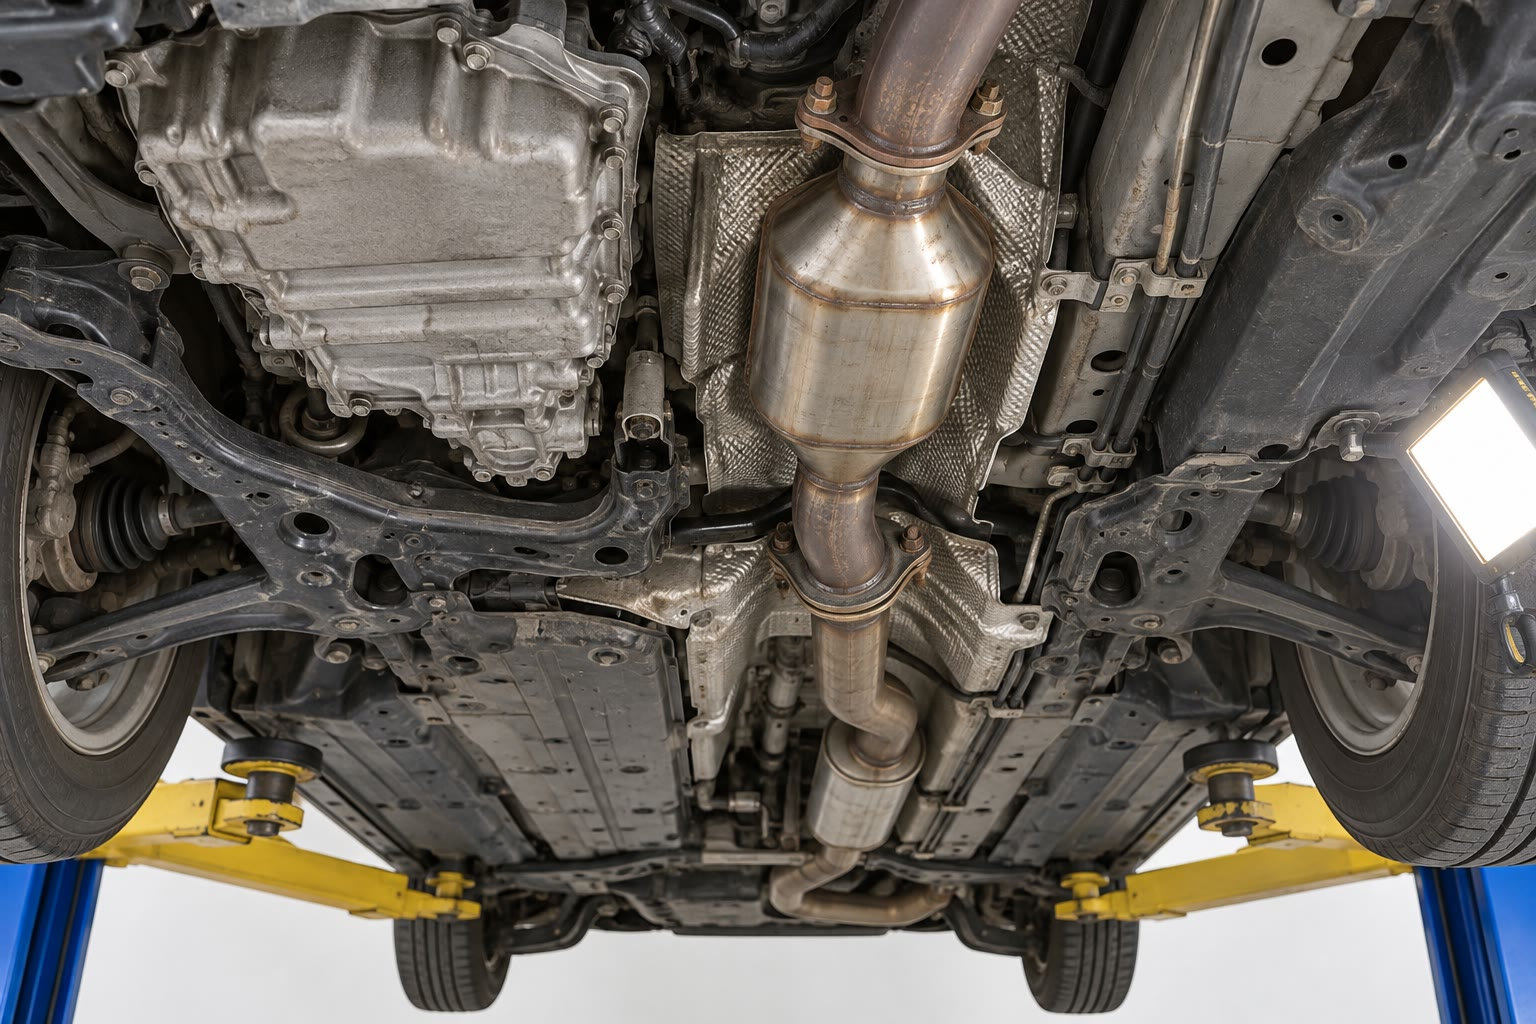
\includegraphics[width=0.5\linewidth]{images/book2/ai/b1-09-catalytic-converter.jpg}

{\small Los bajos de un coche: el cilindro de la línea de escape es un
\omterm{def:b1:elementary-steps:catalyst}{catalizador} de tres vías, un \omterm{def:b1:elementary-steps:catalyst}{catalizador} heterogéneo en cuya superficie
metálica reaccionan los gases de escape.}
\end{omfigure}

\begin{definition}[Control cinético y control termodinámico]\label{def:b1:elementary-steps:control}
Cuando un reactivo puede dar dos productos por caminos competitivos, la
reacción está bajo \emph{control cinético}\index{control cinetico@control cinético} si las
proporciones de productos están fijadas por las \omterm{def:b1:rate-laws:rate}{velocidades de formación}
(domina el producto de barrera más baja), y bajo \emph{control
termodinámico}\index{control termodinamico@control termodinámico} si los caminos son reversibles y el
sistema alcanza el equilibrio (domina el producto más estable).
\end{definition}

\begin{example}[Elegir el producto]\label{ex:b1:elementary-steps:control}
Un reactivo da B por encima de una barrera de \qty{50}{kJ/mol}
($\Delta E =
\qty{-10}{kJ/mol}$) y C por encima de una barrera de \qty{70}{kJ/mol}
($\Delta E =
\qty{-40}{kJ/mol}$). A \qty{300}{K} y tiempos cortos, con \omterm{def:b1:rate-laws:activation-energy}{factores
preexponenciales} iguales, B se forma $\exp(20000/(8.314 \times 300)) \approx
3000$ veces más deprisa que C: el \omterm{def:b1:elementary-steps:control}{control cinético} da B. A temperatura
alta y tiempos largos, B vuelve atrás por encima de su pequeña barrera
inversa, C no, y el sistema termina como C: \omterm{def:b1:elementary-steps:control}{control termodinámico}.
\end{example}

\begin{history}[La catálisis, 1835]
En 1835, el químico sueco Jöns Jacob Berzelius reunió bajo una sola
palabra una docena de observaciones desconcertantes --- el almidón
convertido en azúcar por los ácidos, el peróxido de hidrógeno descompuesto
por los metales, el alcohol oxidado sobre platino --- y llamó
``catalítica'' a la fuerza oculta que actuaba en ellas. Hizo falta la
cinética de finales de siglo, con Wilhelm Ostwald, para definir un
\omterm{def:b1:elementary-steps:catalyst}{catalizador} como una especie que cambia la velocidad de una reacción y no
su equilibrio.
\end{history}

\section{Ejercicios}

\begin{exercise}[$\star$]\label{exo:b1:elementary-steps:1}
Dese la \omterm{def:b1:elementary-steps:elementary-step}{molecularidad} de cada etapa y dígase qué etapas pueden ser
elementales:
(a) $\ce{N2O5 -> NO2 + NO3}$; (b) $\ce{NO + NO3 -> 2NO2}$;
(c) $\ce{2H2 + O2 -> 2H2O}$; (d) $\ce{O + O2 + N2 -> O3 + N2}$.
\end{exercise}

\begin{exercise}[$\star$]\label{exo:b1:elementary-steps:2}
Escríbase la \omterm{def:b1:rate-laws:order}{ley de velocidad} de las \omterm{def:b1:elementary-steps:elementary-step}{etapas elementales} $\mathrm{A} + \mathrm{B} \to
\mathrm{C}$, $2\,\mathrm{A} \to \mathrm{B}$ y $\mathrm{A} \to \mathrm{B} +
\mathrm{C}$. ¿Por qué no puede escribirse la \omterm{def:b1:rate-laws:order}{ley de velocidad} de una
reacción global a partir de su ecuación?
\end{exercise}

\begin{exercise}[$\star$]\label{exo:b1:elementary-steps:3}
En el \omterm{def:b1:elementary-steps:energy-profile}{perfil de energía} de dos etapas dibujado en este capítulo
(intermedio a 30, \omterm{def:b1:elementary-steps:energy-profile}{estados de transición} a 70 y 55 y productos a $-40$, en
\unit{kJ/mol} por encima de los reactivos), identifíquense el intermedio,
los \omterm{def:b1:elementary-steps:energy-profile}{estados de transición} y la \omterm{def:b1:elementary-steps:rds}{etapa determinante de la velocidad}. ¿La
primera etapa es endotérmica o exotérmica?
\end{exercise}

\begin{exercise}[$\star$]\label{exo:b1:elementary-steps:4}
Un \omterm{def:b1:elementary-steps:catalyst}{catalizador} multiplica por $10^4$ la \omterm{def:b1:rate-laws:order}{constante de velocidad} directa de
una \omterm{def:b1:elementary-steps:elementary-step}{etapa elemental}. ¿Por cuánto multiplica la \omterm{def:b1:rate-laws:order}{constante de velocidad}
inversa? ¿Y la constante de equilibrio? ¿Y el tiempo necesario para
alcanzar el equilibrio?
\end{exercise}

\begin{exercise}[$\star\star$]\label{exo:b1:elementary-steps:5}
Para $\mathrm{A} \to \mathrm{B} \to \mathrm{C}$ con $k_1 =
\qty{0.10}{s^{-1}}$ y $k_2 = \qty{0.30}{s^{-1}}$, calcúlense $t_{\max}$ y
la mayor concentración de $\mathrm{B}$, en unidades de $a_0$.
\end{exercise}

\begin{exercise}[$\star\star$]\label{exo:b1:elementary-steps:6}
Para $\mathrm{A} \underset{k_{-1}}{\overset{k_1}{\rightleftharpoons}}
\mathrm{I} \xrightarrow{k_2} \mathrm{P}$, con todas las etapas de orden 1,
aplíquese la \omterm{def:b1:elementary-steps:qssa}{aproximación del estado estacionario} a $\mathrm{I}$ y
demuéstrese que $v =
\frac{k_1k_2}{k_{-1} + k_2}[\mathrm{A}]$. Discútanse los casos $k_2 \gg
k_{-1}$ y $k_2 \ll k_{-1}$.
\end{exercise}

\begin{exercise}[$\star\star$]\label{exo:b1:elementary-steps:7}
Los iones yoduro catalizan la descomposición del peróxido de hidrógeno:
\ce{H2O2 + I- -> H2O + IO-} (lenta) y, después,
\ce{H2O2 + IO- -> H2O + O2 + I-} (rápida). Escríbase la ecuación global,
identifíquense el \omterm{def:b1:elementary-steps:catalyst}{catalizador} y el intermedio, y dese la \omterm{def:b1:rate-laws:order}{ley de
velocidad}.
\end{exercise}

\begin{exercise}[$\star\star$]\label{exo:b1:elementary-steps:8}
Una etapa forma un carbocatión a partir de una molécula neutra, un
proceso muy cuesta arriba. Explíquese, con el postulado de Hammond, por
qué un sustituyente que estabiliza el carbocatión acelera también la
etapa.
\end{exercise}

\begin{exercise}[$\star\star$]\label{exo:b1:elementary-steps:9}
En el \cref{ex:b1:elementary-steps:control}, calcúlese la razón de las
constantes de \omterm{def:b1:rate-laws:rate}{velocidad de formación} de B y de C a \qty{300}{K} y a
\qty{600}{K}. Coméntese.
\end{exercise}

\begin{exercise}[$\star\star\star$]\label{exo:b1:elementary-steps:10}
Un gas $\mathrm{A}$ se descompone tras ser activado por choque con una
molécula cualquiera $\mathrm{M}$: $\mathrm{A} + \mathrm{M} \rightleftharpoons
\mathrm{A}^* + \mathrm{M}$ ($k_1$, $k_{-1}$) y, después, $\mathrm{A}^* \to
\mathrm{P}$ ($k_2$). Con la \omterm{def:b1:elementary-steps:qssa}{aproximación del estado estacionario} para
$\mathrm{A}^*$, hállese $v$ y demuéstrese que la reacción es de orden 1 a
presión alta y de orden 2 a presión baja.
\end{exercise}

\begin{exercise}[$\star\star\star$]\label{exo:b1:elementary-steps:11}
Demuéstrese la fórmula de $[\mathrm{B}](t)$ del
\cref{thm:b1:elementary-steps:consecutive} y trátese el caso particular
$k_1 = k_2 = k$, para el que $[\mathrm{B}] = a_0kt\,\eu^{-kt}$.
\end{exercise}

\begin{exercise}[$\star\star\star$]\label{exo:b1:elementary-steps:12}
La reacción global $\mathrm{A} + 2\,\mathrm{B} \to \mathrm{P} +
\mathrm{C}$ tiene la \omterm{def:b1:rate-laws:order}{ley de velocidad} experimental $v =
k[\mathrm{A}][\mathrm{B}]^2/[\mathrm{C}]$. Propóngase un mecanismo con un
preequilibrio rápido que la explique.
\end{exercise}

\section{Problema: por qué el monóxido de nitrógeno se oxida más deprisa en frío}

\begin{problem}[{Problema de fin de semana --- la oxidación de tercer orden
del monóxido de nitrógeno, un preequilibrio a través del dímero
\ce{N2O2}, el tratamiento del estado estacionario y una \omterm{def:b1:rate-laws:activation-energy}{energía de
activación} aparente negativa}]
\label{pb:b1:elementary-steps:1}
Para \ce{2NO(g) + O2(g) -> 2NO2(g)}, medidas de \omterm{def:b1:rate-laws:initial-rate}{velocidades iniciales} a
\qty{300}{K} dan (velocidades en \unit{mol.L^{-1}.s^{-1}}):
\begin{center}
\begin{tabular}{cccc}
\hline
experimento & $[\ce{NO}]_0$ (mol/L) & $[\ce{O2}]_0$ (mol/L) & $v_0$ \\
\hline
1 & \num{1.0e-3} & \num{1.0e-3} & \num{1.0e-5} \\
2 & \num{2.0e-3} & \num{1.0e-3} & \num{4.0e-5} \\
3 & \num{1.0e-3} & \num{2.0e-3} & \num{2.0e-5} \\
\hline
\end{tabular}
\end{center}
La \omterm{def:b1:rate-laws:order}{constante de velocidad} hallada a \qty{400}{K} es diez veces menor que a
\qty{300}{K}. Tómese $R = \qty{8.314}{J/(mol.K)}$.
El mecanismo propuesto es
\[
  \ce{2NO <=> N2O2} \ \ (k_1, k_{-1}, \text{rápida}), \qquad
  \ce{N2O2 + O2 -> 2NO2} \ \ (k_2, \text{lenta}).
\]

\medskip
\noindent\textbf{Parte I --- La ley observada.}
\begin{enumerate}
  \item Hállense los \omterm{def:b1:rate-laws:order}{órdenes parciales} respecto de \ce{NO} y de \ce{O2}.
  \item Escríbase la \omterm{def:b1:rate-laws:order}{ley de velocidad} y calcúlese $k$ a \qty{300}{K}, con
        su unidad.
  \item ¿Podría ser la reacción una sola etapa trimolecular? Dese un
        argumento.
  \item Calcúlese la \omterm{def:b1:rate-laws:activation-energy}{energía de activación} aparente a partir de las dos
        temperaturas.
  \item ¿Por qué es imposible una \omterm{def:b1:rate-laws:activation-energy}{energía de activación} negativa para una
        \omterm{def:b1:elementary-steps:elementary-step}{etapa elemental}?
  \item Escríbanse las \omterm{def:b1:rate-laws:rate}{velocidades de desaparición} de \ce{NO} y de \ce{O2}
        en función de $v$.
\end{enumerate}

\medskip
\noindent\textbf{Parte II --- El preequilibrio.}
\begin{enumerate}[resume]
  \item Compruébese que las dos etapas suman la reacción global.
        Nómbrese el intermedio.
  \item Dese la \omterm{def:b1:elementary-steps:elementary-step}{molecularidad} de cada etapa.
  \item Escríbase la velocidad de la etapa lenta.
  \item Exprésese $[\ce{N2O2}]$ con la \omterm{def:b1:elementary-steps:pre-equilibrium}{aproximación del preequilibrio}.
  \item Dedúzcase la \omterm{def:b1:rate-laws:order}{ley de velocidad} y compárese con el experimento.
  \item Exprésese la constante observada con $k_1$, $k_{-1}$ y $k_2$.
\end{enumerate}

\medskip
\noindent\textbf{Parte III --- El estado estacionario.}
\begin{enumerate}[resume]
  \item Escríbase $\dd[\ce{N2O2}]/\dd t$ para el mecanismo completo.
  \item Aplíquese la \omterm{def:b1:elementary-steps:qssa}{aproximación del estado estacionario} y exprésese
        $[\ce{N2O2}]$.
  \item Dedúzcase la \omterm{def:b1:rate-laws:order}{ley de velocidad} $v = \dfrac{k_1k_2[\ce{NO}]^2[\ce{O2}]}{k_{-1} +
        k_2[\ce{O2}]}$.
  \item ¿En qué límite se reduce al resultado de la parte II?
  \item ¿En qué se convertirían los órdenes en el límite opuesto?
  \item ¿Qué límite respaldan las medidas de la parte I?
\end{enumerate}

\medskip
\noindent\textbf{Parte IV --- La \omterm{def:b1:rate-laws:activation-energy}{energía de activación} aparente.}
Cada etapa sigue la \omterm{thm:b1:rate-laws:arrhenius}{ley de Arrhenius}, con \omterm{def:b1:rate-laws:activation-energy}{energías de activación} $E_1 =
\qty{2}{kJ/mol}$, $E_{-1} = \qty{40}{kJ/mol}$ y $E_2 =
\qty{15}{kJ/mol}$.
\begin{enumerate}[resume]
  \item Escríbase $\ln k$ en función de los logaritmos de $k_1$, $k_{-1}$
        y $k_2$.
  \item Dedúzcase $E_a = E_1 - E_{-1} + E_2$.
  \item Interprétese: ¿por qué una combinación de \omterm{def:b1:elementary-steps:elementary-step}{etapas elementales}
        puede tener una \omterm{def:b1:rate-laws:activation-energy}{energía de activación} aparente negativa?
  \item Esbócese el \omterm{def:b1:elementary-steps:energy-profile}{perfil de energía}: ¿dónde está el segundo \omterm{def:b1:elementary-steps:energy-profile}{estado de
        transición} respecto de los reactivos \ce{2NO + O2}?
  \item ¿En qué factor cambiaría la velocidad entre 300 y \qty{400}{K}
        con este valor?
  \item Calcúlese la \omterm{def:b1:rate-laws:activation-energy}{energía de activación} aparente a partir de los
        valores de las etapas y compárese con la parte I.
\end{enumerate}
\end{problem}
